\section{Zero-Knowledge Proofs}
In our protocol we wish to use zero-knowledge proofs as a core tool to verify users password.

We explore what ZKPs are on a high level, look at a practical analogy of how they work and also how they are used in real life.
Next we look at what are \textit{interactive proof systems}, the framework of zero-knowledge protocols.
And what is \textit{knowledge complexity}, or how to quantify the information exchanged in an interactive proof system and finally what makes an interactive proof systems zero-knowledge.

\subsection{Introduction}
\textit{Zero-Knowledge Proofs} (ZKPs) are a concept in the field of cryptography, and can be used to prove the validity of mathematical statements. What makes ZKPs particularly interesting is that it can achieve that without revealing any information about why a statement is true.

In mathematics, traditional theorem proofs are logical arguments that establish truth through inference rules of a deductive system based on axioms and other proven theorems.
ZKPs are probabilistic, meaning they \textit{"convince"} the verifier of the validity with a negligible margin of error.
We use the term convince, because ZKPs are not absolute truth, but rather the chance of being \textit{false} is next to zero. The difference in definition is subtle, but we will see what that means in practice further on.

ZKPs were first described by Goldwasser, Micali and Rackoff in \cite{GMR} in 1985. 
They proposed a proof system as a two-party protocol between a \textit{prover} and a \textit{verifier}. It relies on the computational difficulty of the quadratic residuosity problem.
\newpage
\subsubsection{The Strange Cave of Ali Baba}
To help our understanding we will explore the \cite{QJM} The Strange Cave of Ali Baba, a famous analogy for a zero-knowledge protocol from a publication called \textit{"How to explain zero-knowledge protocols to your children"}.

\begin{figure}[h]
	\centering
	\includegraphics[height=6cm]{images/zkp}
	\caption{The Strange Cave of Ali Baba}
	\label{fig:strange-cave-of-alibaba}
\end{figure}

\bigskip

Ali Baba's cave has a single entrance, that splits into two tunnels that meet in the middle where there is a door that can only be opened with a secret passphrase.

\bigskip

Peggy (or Prover) wants to prove to Victor (or Verifier) that she knows the secret passphrase, but she doesn't want to revel the secret nor does she want to reveal her knowledge of the secret to anyone else besides Victor.

\bigskip

To do this they come up with a scheme.
Victor stands in front of cave and faces away from the entrance, to not see Peggy. She enters the cave, and goes into one of the tunnels at random.
Victor looks at the entrance, so he can see both tunnels, and signals Peggy which tunnel to come out from.
Peggy knowing the secret can pass through the door in the middle and emerge from the tunnel requested.

\bigskip

If Peggy didn't know the secret she could fool Victor, only by entering the correct tunnel by chance.
But since Victor is choosing the tunnel at random, Peggy's chance of picking the correct tunnel is 50\%. If Victor were to repeat the process $n$ time, her chances of fooling him become arbitrarily small ($2^{-n}$).

With this process Victor can be convinced that Peggy really knows the secret with a very chance ($1 - 2^{-n}$).

\bigskip

Further more any third party observing the interaction cannot be convinced of the validity of the proof because it cannot be assured that the interaction was truly random. 
For example, Victor could have told Peggy his questions in advance, so Peggy would produce a convincing looking proof.

\subsubsection{Applications}
Most commonly ZKPs were used in authentication and identification systems, as a way to prove knowledge of a secret. 
Recently however there have been a number of new applications in the cryptocurrency and digital identity spaces.

The cryptocurrency Zcash uses a \textit{non-interactive zero-knowledge protocol} zk-SNARK \cite{bowe2018multi} to prove the validity of transactions, without revealing anything about the recipients nor the amount sent.

The cryptocurrency Monero uses a ZKP protocol Bulletproofs \cite{bunz2018bulletproofs}, to achieve anonymous transactions.

\textit{Idemix} \cite{camenisch2002design} an anonymous credential system for interaction between digital identities relies on CL-signatures \cite{camenisch2001efficient} to prove ownership of a credential offline, without the issuing organisation.
Idemix has been implemented in the open-source Hyperledger Indy project.

\newpage
\subsection{Definition}
\subsubsection{Interactive Proof Systems}
An interactive proof system is a proof system in which a \textit{prover} attempts to convince a \textit{verifier} that a statement is true.
The prover and the verifier exchange messages until the verifier is convinced of the proof or not.

\begin{figure}[h]
	\centering
	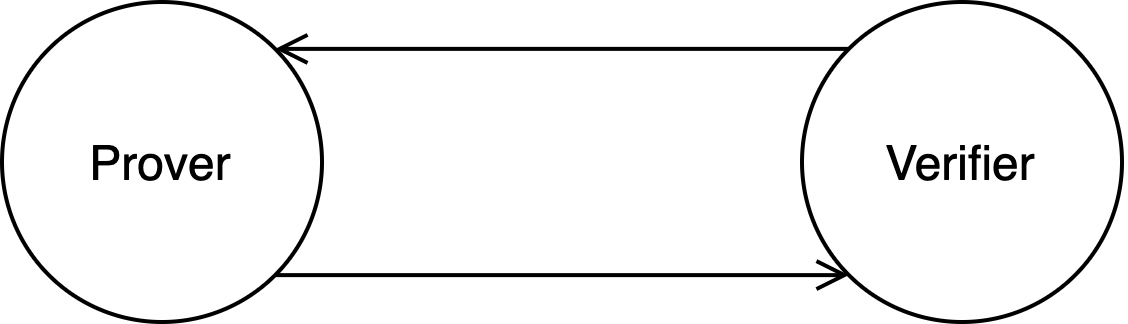
\includegraphics[width=8cm]{images/interactive-proof-system}
	\caption{Interactive Proof System}
	\label{fig:interactive-proof-system}
\end{figure}

The prover is a computationally unbounded polynomial time Turing machine and the verifier is a probabilistic polynomial time Turing machine.
An interactive proof system is defined by properties \textit{completeness} and \textit{soundness}.

\paragraph{Notation}
\begin{description}
	\item $\Pr[A]$: probability of event $A$ happening.
	\item $P(x) = y$: prover $P$, outputs a witness $y$ for statement $x$.
	\item $V(y) = 1$: verifier $V$, analyses witness $y$ and outputs $1$ for valid witness or $0$.
\end{description}

\paragraph{Completeness}

Any honest prover can convince the verifier with overwhelming probability.\\
For $x \in L$ and each $k \in \mathbb{N}$ and sufficiently large $n$;

$$\Pr[x \in L; P(x) = y; V(y) = 1] \ge 1 - \frac{1}{n^k}$$

\paragraph{Soundness}

Any verifier following the protocol will reject a cheating prover with overwhelming probability.\\
For $x \notin L$ and each $k \in \mathbb{N}$ and sufficiently large $n$;

$$\Pr[x \notin L; P(x) = y; V(y) = 0] \ge 1 - \frac{1}{n^k}$$

\subsection{Knowledge Complexity}

\textit{Zero-knowledge proof systems} prove the  membership of $x$ in language $L$, without revealing any additional knowledge (e.g why is $x \in L$).

The essence of zero-knowledge is the idea that what the verifier \textit{sees} is indistinguishable from what can be easily \textit{simulated} on public inputs.
The term \textit{knowledge complexity} quantifies the degrees of indistinguishability of different languages and proof constructions.

The essence of zero-knowledge is the idea that the data the verifier has (from current and past interactions with the prover) is indistinguishable from data that can be \textit{"simulated"} without provers secret information.
For example, if we return to our analogy in the introduction. 
Victor wants to "cheat" and record what he sees to later analyse, or to prove to someone else that Peggy knows the secret.
Victor manages to record which tunnels he calls and from which Peggy emerges, he doesn't record which tunnel Peggy goes into as he is facing away.
Later on Larry and Monica decide to record a similar scheme without knowing the secret.
Larry records himself calling the tunnels and Monica emerging randomly, sometimes she emerges from the correct one other times she doesn't. 
Larry later edits the video to only show the times Monica correctly emerged from the tunnel, as if she knew the secret.
Assuming Larry's video editing skills are good, the videos Larry and Victor recorded are indistinguishable, both videos feature someone calling tunnels and a person emerging. 
While one video records a valid proof and the other one doesn't, there is no information in them from which we could learn that.

\subsubsection{Indistinguishability}
Indistinguishability describes degrees of an inability to distinguish between two random variables $U, V$.
\bigskip
\newline
Let $U = \{U(x)\}$ and $V = \{V(x)\}$ be two families of random variables, where $x$ is from a language $L$, a subset of $\{0, 1\}^*$.
\newline
An algorithm $A(x)$ is given a random sample $x$ from either distribution and will output either $1$ or $0$, depending which distribution it determines the sample originated from.
Distributions become "indistinguishable" as the outputs of the algorithm become uncorrelated to the origin of the sample.

By bounding the \textit{size} of the sample and the \textit{time} given to the algorithm we can obtain different notions of indistinguishability.

%\subsubsection{Indistinguishability of Random Variables} %TODO: Simplify this
%
%Let $U = \{U(x)\}$ and $V = \{V(x)\}$ be two families of random variables, where $x$ is from a language $L$, a particular subset of $\{0, 1\}^*$.
%
%In the framework for distinguishing between random variables, a "judge" is given a sample selected randomly from either $V(x)$ or $U(x)$.
%A judge studies the sample and outputs either a $0$ or a $1$, depending on which distribution he thinks the sample came from.
%
%$U(x)$ essentially becomes "replaceable" by $V(x)$, when $x$ increases and any judges prediction becomes uncorrelated with the origin distribution.


\paragraph{Equality} 
%Given that $U(x)$ and $V(x)$ are equal, they will remain indistinguishable, even if the samples are of arbitrary size and can be studied for an arbitrary amount of time.

If $U(x)$ and $V(x)$ are equal, outputs of a computationally unbounded algorithm will remain uncorrelated with the origin of the sample.

\paragraph{Statistical Indistinguishability} Two random variables are statistically indistinguishable, when the algorithms outputs remain uncorrelated with the origin, given an arbitrary amount of time and a poly-bounded sample size.
\bigskip
\newline
Let $L \subset \{0,1\}^*$ be a language, $U(x)$ and $V(x)$ are statistically indistinguishable on $L$ if,
\bigskip
$$|\Pr [A(x, U) = 1] - \Pr [A(x, V) = 1]| < |x|^{-c}$$ %TODO: Probably not right, check later.
\bigskip
\newline
for $\forall c > 0$, and sufficiently long $x \in L$. 

%\subparagraph{Statistical Indistinguishability} Two random variables are statistically indistinguishable, when given a polynomial sized sample and an arbitrary amount of time, the judges verdict remains meaningless.
%
%\bigskip
%
%Let $L \subset \{0,1\}^*$ be a language, $U(x)$ and $V(x)$ are statistically indistinguishable on $L$ if,
%
%$$\sum_{\alpha \in \{0,1\}^*} |prob(U(x) = \alpha) - prob(V(x) = \alpha) | < |x|^{-c}$$
%
%
%
%for $\forall c > 0$, and sufficiently long $x \in L$. 

\paragraph{Computational Indistinguishability} %TODO: Probably need to clarify the link between poly-time algorithm and poly-sized family of circuits.
Two random variables are computationally indistinguishable, when the poly-time bounded algorithms outputs remain uncorrelated with the origin, given a poly-bounded sample size.
\bigskip
\newline
Let $L \subset \{0,1\}^*$ be a language, poly-bounded families of random variables $U(x)$ and $V(x)$ are computationally indistinguishable on $L$ if for all poly-sized family of circuits $C$, $\forall c > 0$, and a sufficiently long $x \in L$

$$|\Pr[C(U, x) = 1] - \Pr[C(V, x) = 1]|  < |x|^{-c}$$


%\subparagraph{Computational Indistinguishability}%TODO: Simplify this
%
%Two random variables are computationally indistinguishable, if judges verdict remains meaningless given a polynomial sized sample and polynomial amount of time.
%
%\bigskip
%
%Let $L \subset \{0,1\}^*$ be a language, poly-bounded families of random variables $U(x)$ and $V(x)$ are computationally indistinguishable on $L$ if for all poly-sized family of circuits $C$, $\forall c > 0$, and a sufficiently long $x \in L$
%
%$$|P(U, C, x) - P(V, C, x)| < |x|^{-c}$$
%
%Any two families that are \textit{computationally indistinguishable} are considered  \textit{indistinguishable} in general.

\subsubsection{Approximability of Random Variables}%TODO: Simplify this

The notion of approximability described the degree to which a random variable $U(x)$ can be "generated" by a probabilistic Turing machine $M$, generating a probability distribution $M(x)$.
\bigskip
\newline
A random variable $U(x)$ is \textit{perfectly approximable} if there exists a probabilistic Turing machine $M$, such that for $x \in L$, $M(x)$ is \textit{equal} to $U(x)$.
\newline
$U(x)$ is statistically or computationally approximable if $M(x)$ is statistically or computationally indistinguishable from $U(x)$.

\bigskip

Generally speaking when saying a family of random variables $U(x)$ is \textit{approximable} we mean that it is \textit{computationally} approximable.

\subsubsection{Definition of Zero-Knowledge}

Zero-knowledge is a degree of protocols knowledge complexity at which no meaningful information can be extracted by the verifier or any third party observer.
\bigskip
\newline
A protocol is zero-knowledge if the verifiers "view" is approximable by a simulator $S$.
A verifiers view is all data that was exchanged with the prover, a cheating verifier's view might have extra information (e.g a history of previous interactions).

A protocols is perfectly zero-knowledge if the view is perfectly approximable for all verifiers.
Statistical or computational zero-knowledge is obtained by statistical or computational approximability.